\section{The idea behind web scraping}
\subsection{APIs vs. web scraping}

\begin{frame}{Ways to collect online data}
  \begin{enumerate}
  \item Download existing datasets (that's trivial\ldots)
  \item Use an API (relatively easy)
  \item Web scraping (anything between easy and extremely difficult)
  \end{enumerate}
\end{frame}


\begin{frame}{APIs vs web scraping}
  \begin{columns}[t]
    \column{.5\textwidth}
    \begin{block}{APIs}
      \begin{itemize}
      \item $+$ structured (or at least semi-structured) data (JSON)
      \item $+$ little programming effort needed
      \item $-$ not always available; or restrictions apply
      \item $-$ no guarantee it looks like what a human would see
      \end{itemize}
    \end{block}
    \pause
    \column{.5\textwidth}
    \begin{alertblock}{web scraping}
      \begin{itemize}
      \item $-$ unstructured data (HTML text)
      \item $-$ (potentially) much programming effort needed
      \item $+$ in principle always* possible
      \item $+$ see what a human user would see*
      \end{itemize}
    \end{alertblock}
  \end{columns}

* \footnotesize{Don't get too excited. With dynamic websites that use a lot of stuff like JavaScript, Cookie Walls, etc., this can be difficult to unfeasible.}
\end{frame}


\begin{frame}[standout]
  If there's an API, you want to use the API (either directly with the \texttt{requests} package or via a so-called wrapper (a package that makes using a specific API even easier).

  Otherwise, consider using web scraping.

\end{frame}

\subsection{From HTML to structured data}


\begin{frame}
Let's have a look at some websites and understand the underlying structure.
\vspace{1cm}
\pause
\begin{alertblock}{Websites change constantly!}
The examples are meant to illustrate the principles and approaches and are \emph{not} meant as a practical guide for scraping specific websites. Websites change their structure quite regularly, and you cannot assume that scraping code written once keeps working in the future.
\end{alertblock}
\footnotesize{Except, of course, the simplified example at \url{https://cssbook.net/d/eat/} -- that one will be kept unchanged ;-)}
\end{frame}


\question{Do you know some HTML?}


{\setbeamercolor{background canvas}{bg=black}
\begin{frame}[plain]
\makebox[\linewidth]{
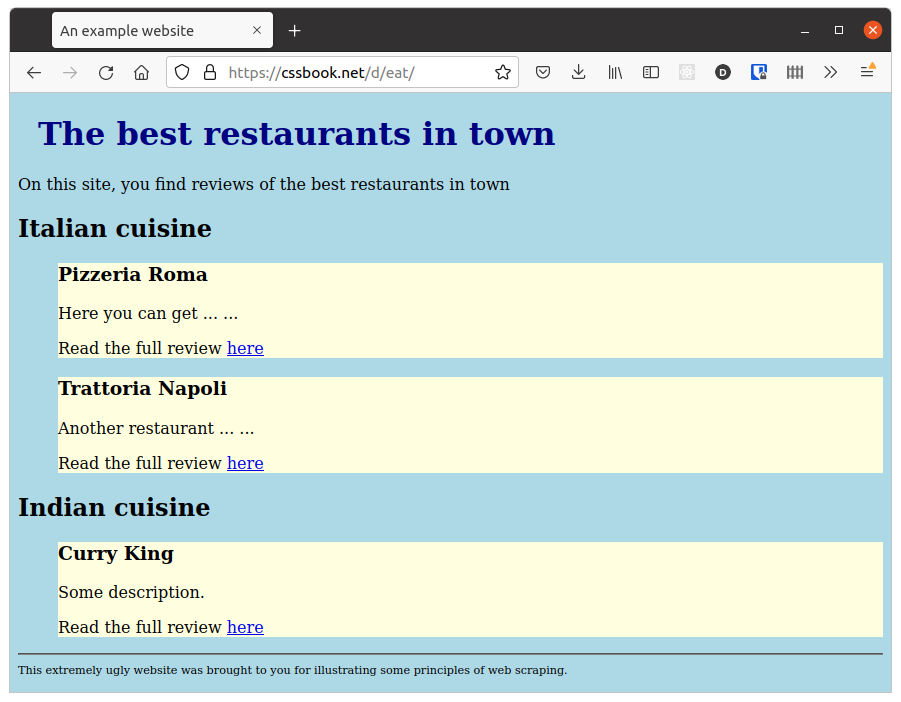
\includegraphics[width=\paperwidth,height=\paperheight,keepaspectratio]{scraping-eat-browser.png}}
\end{frame}
}

\begin{frame}[plain]
If you view the underlying source code (depending on your browser, sth like ``View Source'', ``View Page Source'', or \texttt{CTRL-U})\ldots

\end{frame}
{\setbeamercolor{background canvas}{bg=black}
\begin{frame}[plain]
\makebox[\linewidth]{
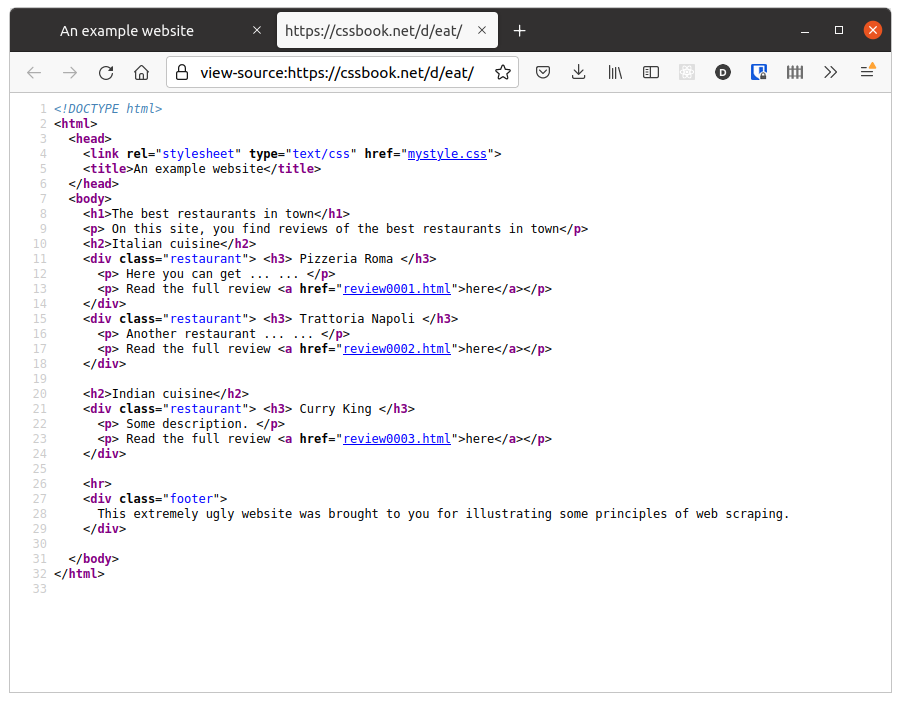
\includegraphics[width=\paperwidth,height=\paperheight,keepaspectratio]{scraping-eat-source.png}}
\end{frame}
}


\begin{frame}[plain]
You can get an even more comfortable view of the source code using the ``Inspect element'' function:

\end{frame}
{\setbeamercolor{background canvas}{bg=black}
\begin{frame}[plain]
\makebox[\linewidth]{
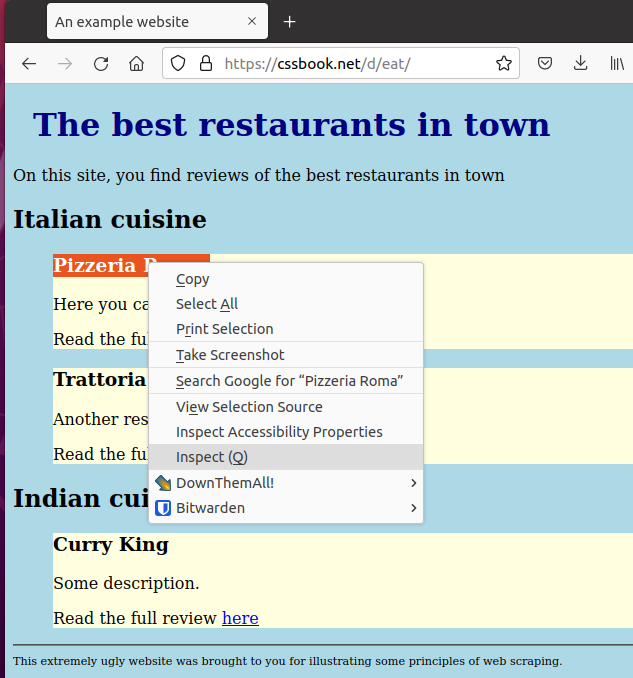
\includegraphics[width=\paperwidth,height=\paperheight,keepaspectratio]{scraping-eat-inspect1.png}}
\end{frame}
\begin{frame}[plain]
\makebox[\linewidth]{
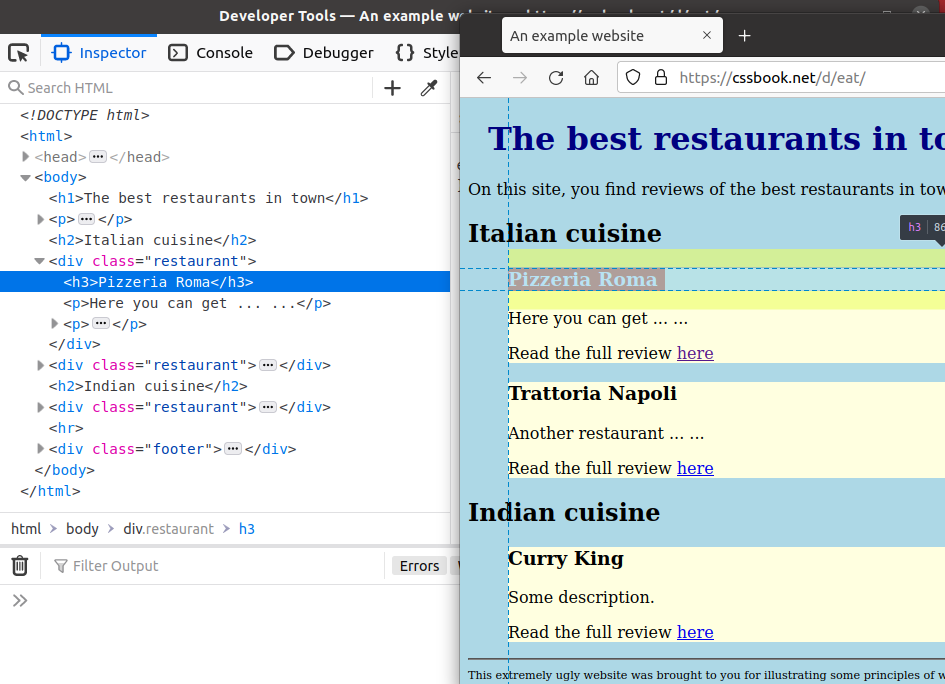
\includegraphics[width=\paperwidth,height=\paperheight,keepaspectratio]{scraping-eat-inspect2.png}}
\end{frame}
}





\begin{frame}{Let's make a plan!}
\begin{block}{Which elements from the page do we need?}
\begin{itemize}
\item What do they mean?
\item How are they represented in the source code?
\end{itemize}
\end{block}
\begin{block}{How should our output look like?}
\begin{itemize}
\item What \emph{lists} do we want?
\item \ldots
\end{itemize}
\end{block}
And how can we achieve this?
\end{frame}


\question{Go to \url{https://cssbook.net/d/eat} and explore which elements we may need!}


\begin{frame}[fragile]{1. Retrieve the web page}
\begin{minted}{python}
import requests
r = requests.get("https://cssbook.net/d/eat/")
htmlsource = r.text   # that's all!

# Additional verification if needed:
# (a) this should print exactly the source code in the browser
print(htmlsource)

# (b) opening test.html in your browser should show the same page
# as you would have gotten with a "File/Save As" in the browser
with open("test.html", mode="w") as f:
    f.write(r.text)
\end{minted}
You see that it's exactly the same as with retrieving data from a JSON-based API -- just that we use  \texttt{.text} instead of \texttt{.json} in line 3.
\end{frame}

\begin{frame}[fragile]{2. Parse the HTML code}
We could now use regular expressions to extract the relevant information
\pause
\begin{minted}{python}
import re    
re.findall(r"<h3>(.*?)</h3>", htmlsource)

# returns [' Pizzeria Roma ', ' Trattoria Napoli ', ' Curry King ']
\end{minted}
\end{frame}

\begin{frame}{2. Parse the HTML code}
  But:
  \begin{itemize}
  \item difficult for more complex pages
  \item error-prone
  \item hard to consider all edge cases (what about tags in tags? linebreaks? \ldots)
  \end{itemize}

  \pause

  \begin{alertblock}{Others have written these regular expressions for you!}
Very few edge cases aside (broken pages, for instance), you do not write these (low-level) regular expressions yourself but use existing packages that let you describe the position of some content within a HTML file with an easier (high-level) syntax, so-called CSS Selectors and/or XPATHs (two new languages next to regexp, yeah!\footnote{I promise they are easier!})
\end{alertblock}


\end{frame}





\section{XPATHs and CSS Selectors}

\subsection{HTML documents as trees}

\begin{frame}{HTMl documents are hierarchical}
  \begin{itemize}
  \item tags are opened (\texttt{<b>}) and closed  (\texttt{</b>})
  \item tags are nested
  \item hence, we can represent them as a tree
  \end{itemize}
\footnotesize{It's also called a DOM-tree (Document Object Model)}
\end{frame}

\question{Go back to your browser window inspecting our example page. Can you see this back?}


\begin{frame}[plain]
  \tiny
  \url{https://en.wikipedia.org/wiki/Document_Object_Model}
  \makebox[\linewidth]{
    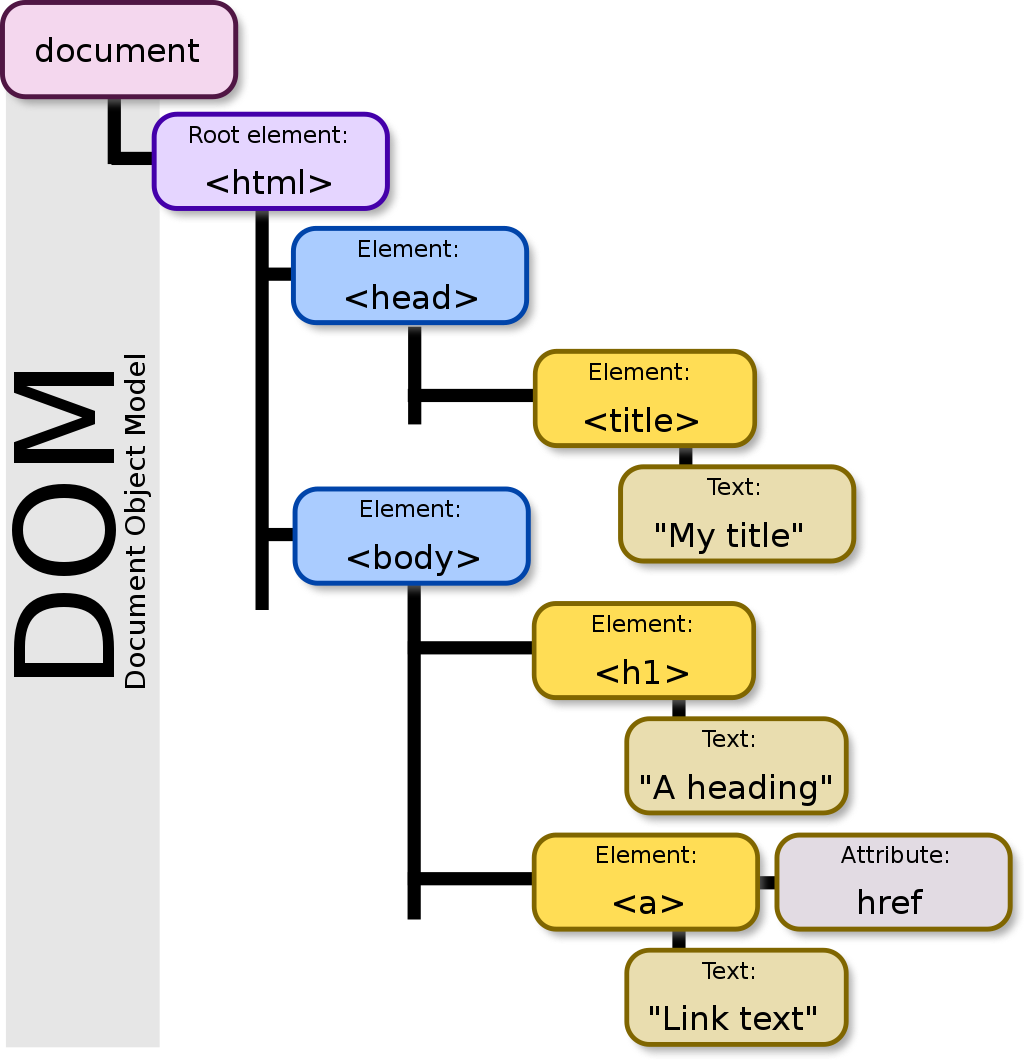
\includegraphics[width=\paperwidth,height=\paperheight,keepaspectratio]{dom.png}}
\end{frame}



\begin{frame}[standout]
We can use an XPATH to denote a position in the tree (``how to traverse the tree, starting from the root'').
\end{frame}


\begin{frame}[standout]
Alternatively, we can use CSS Selectors to select specific tags and/or attributes
\end{frame}



\begin{frame}[fragile]{Back to our example}
We now have much better tools!

\begin{minted}{python}
from lxml.html import fromstring

tree = fromstring(htmlsource)

# instead of re.findall(r"<h3>(.*?)</h3>", htmlsource)
# we now have two easier options:
print([e.text_content() for e in tree.xpath("//h3")])
print([e.text_content() for e in tree.cssselect("h3")])

# Note that e is an element with many methods and properties.
# Try out grabbing the first one and use TAB completion:
test = tree.cssselect("h3")[0]
test.#press TAB
\end{minted}

\end{frame}


\begin{frame}[standout]
Let's look at an overview of the syntax: \url{https://cssbook.net/chapter12.html\#tab:cssselect}
\end{frame}



\begin{frame}[fragile]{CSS Selector vs XPATH }
Two equivalent examples:
\begin{minted}{python}
# we extract all relevant elements using their XPATH
elements = tree.xpath('//div[@class="restaurant"]')

# alternatively, we can use their CSS selector:
elements2 =  tree.cssselect("div.restaurants")

assert elements==elements2
\end{minted}

\tiny{If you want to use CSS selectors, you may need to \texttt{pip install cssselect} first}
\end{frame}



\begin{frame}[fragile]{CSS Selector vs XPATH }
\begin{itemize}
	\item partly a matter of personal preferences
	\item Table 12.1 in the book shows both
	\item CSS selectors are often easier to write (and more modern)
	\item XPATHs are more straight-forward for describing the hierarchical position of an object
	\item there are some cases that cannot be described as CSS selector (in particular, arbiraty attributes)
\end{itemize}
$\Rightarrow$ Many people us CSS selectors by default and restort to XPATHs if necessary
\end{frame}













\section{Scaling up}




\begin{frame}[fragile]{But this was on \emph{one} page only, right?}
Next step: Repeat for each relevant page.

\begin{block}{Possibility 1: Based on url schemes}
	If the url of one review page is \url{https://www.hostelworld.com/hosteldetails.php/ClinkNOORD/Amsterdam/93919/reviews?page=2}

\ldots then the next one is probably?
\end{block}

\pause

$\Rightarrow$ you can construct a list of all possible URLs:

\begin{lstlisting}
MAXPAGES = 20
baseurl = 'https://www.hostelworld.com/hosteldetails.php/ClinkNOORD/Amsterdam/93919/reviews?page='
allurls = [f"baseurl{i}" for i in range(1,MAXPAGES+1)]
\end{lstlisting}	
	
\end{frame}



\begin{frame}[fragile]{But this was on \emph{one} page only, right?}
  Next step: Repeat for each relevant page.
  
  \begin{block}{Possibility 2: Based on XPATHs or CSS Selectors}
    Use XPATH to get the url of the next page (i.e., to get the link that you would click to get the next review)
  \end{block}
	
\end{frame}


\begin{frame}{Recap}
\begin{block}{General idea}
\begin{enumerate}
\item Identify each element by its XPATH or CSS Selector (look it up in your browser) 
\item Read the webpage into a (loooooong) string
\item Use the XPATH  or CSS Selectors to extract the relevant text into a list (with a module like lxml)
\item Do something with the list (preprocess, analyze, save)
\item Repeat
\end{enumerate}
\end{block}
\end{frame}


\begin{frame}{General remarks}
  \begin{block}{There is often more than one way to specify an XPATH or CSS Selector}
    \begin{enumerate}
    \item It's about finding a description that is not too general (e.g., each H3) tag but also not too specific (the second H3 tag nested in the first div nested in\ldots)
      \item (a bit like the precision-recall trade-off we discussed)
      \item Look into the structure of the HTML code, for example with ``Inspect Element'' and use that information to play around with different possibilities
    \end{enumerate}
  \end{block}
\end{frame}



\begin{frame}[standout]
Let's look at the example at \url{https://github.com/uvacw/teaching-bdaca/blob/main/modules/scraping/scraping.ipynb}
\end{frame}


\subsection{Avanced techniques}

\begin{frame}[standout]
We could talk endlessly about all the following techniques, but it's probably better to just look at them once you need them. But a quick overview is always good!
\end{frame}

\begin{frame}[standout]
See especially Chapter 12.3: Authentication, Cookies, and Sessions
\end{frame}

\begin{frame}{Dynamic vs static pages}
  \begin{itemize}
  \item Modern pages often use techniques like JavaScript to load or refresh content -- in this case, the HTML response you got via \texttt{requests} does not contain the final content
  \item (it cannot -- as you do not use a browser that could run the JavaScript)
  \item Solution: Literally use a browser (via Selenium)
  \end{itemize}
\end{frame}



\begin{frame}{Which browser am I (pretending to be)?}
  \begin{itemize}
  \item When a HTTP request is made, it contains a header with meta-information
  \item One is the ``User-Agent'' (name and version of sender)
  \item You may want to set this specifically to pretend to be a specific browser (maybe even a mobile one!)
  \end{itemize}
\end{frame}



\begin{frame}{Sessions and Cookies}
  \begin{itemize}
  \item Sometimes, it may be necessary to explicitly store and/or set cookies
  \item You can do this with \emph{Sessions} and \emph{Cookie Jars} in \texttt{requests}
  \item Or you let your browser handle it via Selenium
  \end{itemize}
\end{frame}
